% =============================================================
% RAR -- Master paper file
% KDD 2026 submission (research track, anonymous, double-blind)
% Built 2026-07-09 from intro_final + background + method +
%   eval_scaffold + related_work + conclusion.
%
% Compile (Overleaf or local with TeX Live):
%   pdflatex paper
%   bibtex paper
%   pdflatex paper
%   pdflatex paper
% =============================================================

\documentclass[sigconf,review,anonymous]{acmart}
%% KDD 2026 research track: double-column format.
%% "The recommended setting for LaTeX is:
%%   \documentclass[sigconf,review]{acmart}"

% --- font encoding ---
\usepackage[T1]{fontenc}
\usepackage[utf8]{inputenc}

% --- math font (acmart requires Libertine; only load libertinus-type1 for missing glyphs) ---
\IfFileExists{libertinus-type1.sty}{\usepackage{libertinus-type1}}{}
% If \Bbbk throws "already defined", comment out the line above.

% --- packages ---
\usepackage{booktabs}
\usepackage{array}
\usepackage{amsmath}
\usepackage{graphicx}
\usepackage{xcolor}
\usepackage{tikz}
\usetikzlibrary{positioning, arrows.meta, shapes.geometric, fit, calc, backgrounds}
\usepackage[ruled,linesnumbered]{algorithm2e}

% --- RAR palette (Paul Tol bright, consistent with figure files) ---
\definecolor{ptblue}{HTML}{4477AA}
\definecolor{ptcyan}{HTML}{66CCEE}
\definecolor{ptgreen}{HTML}{228833}
\definecolor{ptred}{HTML}{EE6677}
\definecolor{ptgrey}{HTML}{BBBBBB}

% --- CCS concepts (ACM requirement) ---
\begin{CCSXML}
<ccs2012>
 <concept>
  <concept_id>10003033.10003079.10003084</concept_id>
  <concept_desc>Security and privacy~Network security</concept_desc>
  <concept_significance>500</concept_significance>
 </concept>
 <concept>
  <concept_id>10010147.10010257.10010258.10010261</concept_id>
  <concept_desc>Computing methodologies~Transfer learning</concept_desc>
  <concept_significance>500</concept_significance>
 </concept>
 <concept>
  <concept_id>10003033.10003079.10011665</concept_id>
  <concept_desc>Networks~Traffic classification</concept_desc>
  <concept_significance>300</concept_significance>
 </concept>
</ccs2012>
\end{CCSXML}

\ccsdesc[500]{Security and privacy~Network security}
\ccsdesc[500]{Computing methodologies~Transfer learning}
\ccsdesc[300]{Networks~Traffic classification}

% --- keywords (ACM requirement) ---
\keywords{Encrypted Traffic Classification, Class-Incremental Learning, Knowledge Distillation, Reconstruction-Aware Routing}

% --- metadata ---
\title{RAR: Reconstruction-Aware Routing for Old/New Balancing\\in Encrypted Traffic Class-Incremental Learning}
\author{Anonymous}
\affiliation{\institution{Anonymous Institution}\country{}}
\date{}

\raggedbottom
\begin{document}

% --- abstract (BEFORE \maketitle per acmart requirement) ---
% !TEX root = paper.tex
% =============================================================
% RAR -- Abstract v0
% Source-of-truth: project_context.md (binding constraints).
% Stage 3 of paper-writing skill. Written LAST per Principle 1.
% Last updated: 2026-07-12
%
% Targets ~200-250 words. Locks:
%   - Headline: forgetting 35.5%--67.5%; mix up to 11.7 pp
%   - Six datasets
%   - Core signal: reconstruction-based old/new compatibility
%   - Design spine (implicit): recon -> routing -> dual heads -> calibration
%
% Conventions:
%   - KDD venue: no \smartparagraph.
%   - Zero hedging, active voice, no em-dashes.
%   - Headline numbers anchored to §4 evaluation.
% =============================================================

\begin{abstract}
Encrypted traffic classification identifies applications and services without inspecting packet payloads, supporting network security, service management, and traffic measurement. Modern representations perform strongly on static, closed-set benchmarks. In practice, however, encrypted-traffic classifiers must continually absorb emerging applications and services without retaining all historical training data. This class-incremental setting is especially challenging because different flows from the same application can exhibit substantial variation, whereas flows from different applications can appear similar due to shared protocols, cloud services, or third-party components. Consequently, compatibility with previously learned class representations varies across flows, yet existing replay and distillation methods typically use fixed global weights and cannot adjust preservation and acquisition accordingly. This limitation calls for a per-flow signal of compatibility with historical traffic patterns. We find that an autoencoder fitted to frozen representations of replayed historical traffic tends to reconstruct old-class flows with lower error than newly arriving flows. Based on this observation, we propose Reconstruction-Aware Routing (RAR), which converts reconstruction error into a continuous per-flow old/new compatibility score. The same score controls both incremental optimization, by weighting preservation and acquisition losses, and inference, by softly combining a frozen historical-class path with a trainable new-class path; logit calibration then supports joint prediction over a unified traffic-class space without task identifiers. Experiments on six public encrypted-traffic datasets show that RAR reduces forgetting by 35.5\%--67.5\% over the evaluated classical CIL baselines and improves mixed-class accuracy by up to 11.7 percentage points. Component, multi-step, and replay-budget studies further support reconstruction-aware old/new balancing.
\end{abstract}

\maketitle

% --- numbered sections ---
% !TEX root = paper.tex
% =============================================================
% RAR -- Final Introduction v0
% Source-of-truth: project_context.md (binding constraints).
% Stage 3 of paper-writing skill. Written from scratch per Principle 1.
% Last updated: 2026-07-09
%
% Differs from intro_draft0.tex in:
%   - Key Abstraction now opens with the coined term "knowledge
%     ownership estimation" rather than introducing it tentatively.
%   - Contributions are claim-first with embedded headline numbers.
%   - Results Preview anchors the closing with the locked headline.
%   - Outline paragraph added at the end.
%
% The Draft 0 introduction (intro_draft0.tex) remains as reference.
% On integration: replace intro_draft0.tex with this file and delete
% the draft. Verify all headline numbers against the final tables.
% =============================================================

\section{Introduction}

% Stakes: problem-first, specific actors. Principle 7: domain before
% method. The ML/AI component enters at the Key Abstraction.
Encrypted-traffic classifiers identify applications and threats from packet metadata, length distributions, and timing patterns alone, and the set of classes they must recognize grows continuously. New applications launch, new malware families appear, and each addition forces the classifier to recognize a class it has never seen. Operators run these classifiers under tight latency budgets and cannot retrain from scratch on every addition; the retraining cost grows with the class history.

% Problem Gap: structural, not quantitative. Three gaps are LOCKED
% in project_context.md and named here to bridge to §3.
Class-incremental learning (CIL) targets this need by adding classes without retraining on the full history. Existing CIL methods, including LwF~\cite{li2017lwf}, iCaRL~\cite{rebuffi2017icarl}, BiC~\cite{wu2019bic}, and DER~\cite{yan2021der}, mitigate forgetting through two mechanisms: replaying a small buffer of historical samples and distilling the old model into the new one. Applied to encrypted traffic, three structural gaps remain open. First, expanding the classification head makes old and new classes compete for one shared decision boundary. Second, uniform distillation treats every sample identically, regardless of whether it carries old or new knowledge. Third, replay depends on a limited buffer that cannot represent the full old-class distribution.

% Key Abstraction: the coined term appears prominently. Per
% rhetorical_moves.md, this move appears ONLY in final versions and is
% discovered through writing. The term "knowledge ownership estimation"
% is the paper's intellectual core.
We observe that an autoencoder fitted to frozen features of replayed old samples tends to reconstruct old-class samples with lower error than new-class samples. Reconstruction error therefore provides an input-dependent score of compatibility with the replay-derived old-feature manifold. We call this per-input signal \emph{knowledge ownership estimation}.

% Design Intuition: one-paragraph mental model. The design spine
% (knowledge ownership estimation -> soft routing -> dual knowledge
% paths -> calibration) is the single line that organizes §3.
RAR (Reconstruction-Aware Routing) turns the ownership score into a soft routing weight over two classification paths: a frozen old-knowledge path inherited from the preceding step and a trainable head for the arriving classes. Both paths contribute to every prediction, weighted by the sample's estimated old/new score, and a logit calibration layer unifies their outputs into a joint prediction over all seen classes. A reconstruction temperature $\tau$ controls routing softness: small $\tau$ approaches deterministic path selection; large $\tau$ smoothly fuses both paths. The design follows a single line: knowledge ownership estimation, soft routing, dual knowledge paths, calibration.

% Contributions: numbered, claim-first. Each item is a claim, not a
% process description. "We show" preferred over "We propose".
We make four contributions.
\begin{enumerate}
  \item \textbf{Sample-level knowledge ownership estimation.} We derive an old/new routing score from each sample's reconstruction error, enabling sample-aware knowledge balancing beyond uniform knowledge transfer.
  \item \textbf{Dual-head knowledge path decoupling.} We route old and new knowledge paths to separate heads, removing the shared-classifier competition that causes forgetting.
  \item \textbf{Logit calibration over dual knowledge paths.} We calibrate the two heads' outputs into a unified classification space, raising mixed-class accuracy by 2.3 percentage points (from 87.82\% to 90.12\%) over an uncalibrated dual-head baseline.
  \item \textbf{Validation across six encrypted-traffic datasets.} RAR reduces forgetting by 35.5\%--67.5\% and improves mixed-class accuracy by up to 11.7 percentage points over the strongest classical CIL baseline (Adapter) on six public datasets (NUDT-Mobile, CIC-DoHBrw, CIC-IoT2023, CSTNET-TLS1.3, ISCX-Tor, EBSNN-WebApp). A complementary study shows that naive incremental forgetting persists across nine traffic-classification backbones.
\end{enumerate}

% Results Preview: anchors the introduction with the locked
% headline numbers. Outlines the rest of the paper so the reader knows
% what each section delivers.
The remainder of this paper evaluates the contribution. \S\ref{sec:background} formalizes the encrypted-traffic CIL problem and its three structural gaps. \S\ref{sec:method} presents RAR's mechanism, from reconstruction error through soft routing to calibration, and closes with a training algorithm (Algorithm~1). \S\ref{sec:eval} reports empirical evidence on six datasets: RAR against classical CIL strategies on ET-BERT, a backbone study confirming that naive forgetting persists across nine encoders, a component ablation, and robustness under multi-step increments and tight replay budgets. \S\ref{sec:related} positions RAR against prior work. \S\ref{sec:conclusion} summarizes the contributions, limitations, and future directions.

% !TEX root = paper.tex
% =============================================================
% RAR -- Background and Problem Setup v0
% Source-of-truth: project_context.md (binding constraints).
% Stage 3 of paper-writing skill. Draft 0 intro frozen 2026-07-09.
% Last updated: 2026-07-09
%
% Three structural gaps are LOCKED 2026-07-09 :
%   (i)   shared classifier competition from head expansion
%   (ii)  knowledge-unaware distillation (uniform)
%   (iii) limited replay representation
%
% Conventions:
%   - KDD venue: integrated related work, colon-style subtitles,
%     no \smartparagraph, no em-dashes.
%   - Headings are claims. Topic sentences assert claims.
%   - Cite prior work where applicable; carry forward from §1.
% =============================================================

\section{Preliminaries}\label{sec:background}

% Section opener: claim-first. The three structural gaps that follow
% are the motivation for RAR's design (§3). Tight to ~1 page.

\subsection{The Encrypted-Traffic CIL Setup}

% Topic sentence 1: formalize the problem
We formalize the problem as class-incremental learning (CIL). At the base step, we train on $K_0$ classes. At each incremental step, $K_i$ new classes arrive with a small replay buffer of old samples.

% Topic sentence 2: incremental-step objective
At the incremental step $T_i$ the classifier must satisfy two competing objectives. It must acquire the new classes with high accuracy, and it must retain the old classes despite the head-expansion operation that adds $K_i$ output dimensions to the classification layer. The replay buffer typically holds a fixed small number of samples per old class, which is the only bridge between the base step and the incremental step.

\begin{figure*}[t]
\centering
% =============================================================
% RAR -- Figure 3: Class-incremental learning setup in encrypted traffic
% Label: fig:cil-setup
% Used in: §2.1 The encrypted-traffic CIL setup.
% Format: input-style (no \documentclass). \input{} from paper.tex.
%   For standalone visual preview, wrap in
%     \documentclass[border=5pt]{standalone}
%     \usepackage{tikz} \usetikzlibrary{...}
%     \definecolor{ptblue}{HTML}{4477AA} ... (palette)
% Color palette: Paul Tol bright (matches figures/fig_*.tex).
% =============================================================

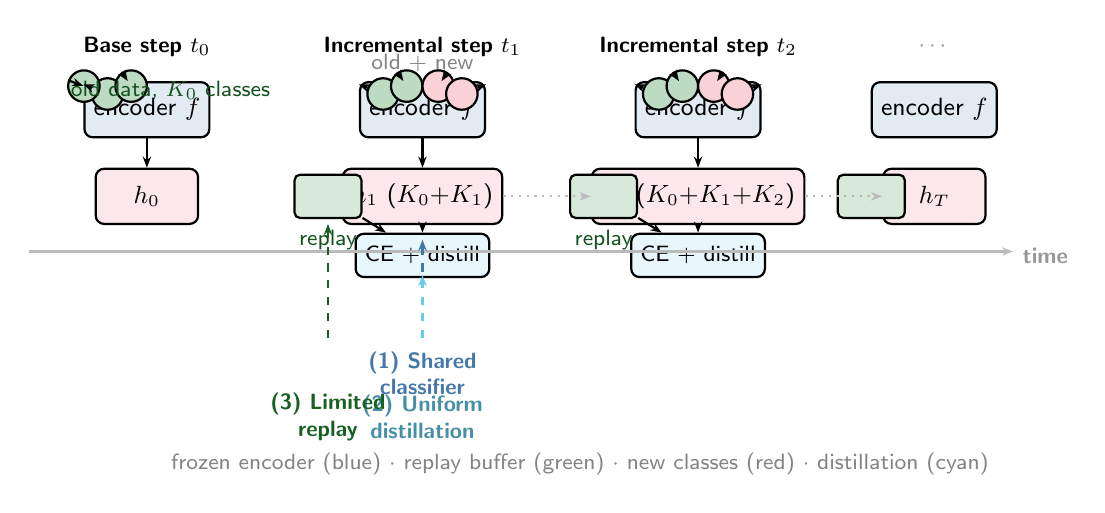
\begin{tikzpicture}[
    node distance=0.4cm and 0.5cm,
    enc/.style={rectangle, draw, thick, rounded corners=3pt,
                minimum width=1.1cm, minimum height=0.7cm,
                font=\small\sffamily, align=center, fill=ptblue!15},
    head/.style={rectangle, draw, thick, rounded corners=3pt,
                 minimum width=1.6cm, minimum height=0.7cm,
                 font=\small\sffamily, align=center, fill=ptred!15},
    buffer/.style={rectangle, draw, thick, rounded corners=2pt,
                   minimum width=0.85cm, minimum height=0.55cm,
                   font=\footnotesize\sffamily, fill=ptgreen!18},
    loss/.style={rectangle, draw, thick, rounded corners=3pt,
                 minimum width=1.2cm, minimum height=0.55cm,
                 font=\footnotesize\sffamily, fill=ptcyan!15},
    sample/.style={circle, draw, thick, inner sep=1pt,
                   minimum size=0.4cm, font=\footnotesize\sffamily},
    oldsample/.style={sample, fill=ptgreen!30},
    newsample/.style={sample, fill=ptred!30},
    arrow/.style={-{Stealth[length=4pt]}, thick},
    gaparr/.style={-{Stealth[length=4pt]}, thick, dashed},
    small/.style={font=\footnotesize\sffamily},
    smallbf/.style={font=\footnotesize\sffamily\bfseries},
]

% ============== base step t0 ==============
\node[smallbf] at (0,2.6) {Base step $t_0$};
\node[enc] (e0) at (0,1.8) {encoder $f$};
\node[head, minimum width=1.3cm] (h0) at (0,0.7) {$h_0$};
\node[oldsample] (s0a) at (-0.5,2.0) {};
\node[oldsample] (s0b) at (-0.2,2.1) {};
\node[oldsample] (s0c) at (-0.8,2.1) {};
\node[small, color=ptgreen!60!black] at (0.3,2.05) {old data, $K_0$ classes};

\draw[arrow] (s0a) -- (e0);
\draw[arrow] (s0b) -- (e0);
\draw[arrow] (s0c) -- (e0);
\draw[arrow] (e0) -- (h0);

% ============== incremental step t1 ==============
\node[smallbf] at (3.5,2.6) {Incremental step $t_1$};
\node[enc, minimum width=1.0cm] (e1) at (3.5,1.8) {encoder $f$};
\node[head, minimum width=2.0cm] (h1) at (3.5,0.7) {$h_1$ ($K_0{+}K_1$)};
\node[buffer] (b1) at (2.3,0.7) {};
\node[small, color=ptgreen!60!black] at (2.3,0.15) {replay};
\node[oldsample] (s1a) at (3.0,2.0) {};
\node[oldsample] (s1b) at (3.3,2.1) {};
\node[newsample] (s1c) at (3.7,2.1) {};
\node[newsample] (s1d) at (4.0,2.0) {};
\node[small, color=ptgrey!70!black] at (3.5,2.4) {old + new};

\node[loss] (l1) at (3.5,-0.05) {CE + distill};

\draw[arrow] (s1a) -- (e1);
\draw[arrow] (s1b) -- (e1);
\draw[arrow] (s1c) -- (e1);
\draw[arrow] (s1d) -- (e1);
\draw[arrow] (e1) -- (h1);
\draw[arrow] (h1) -- (l1);
\draw[arrow] (b1) -- (l1);

% ============== incremental step t2 ==============
\node[smallbf] at (7.0,2.6) {Incremental step $t_2$};
\node[enc, minimum width=1.0cm] (e2) at (7.0,1.8) {encoder $f$};
\node[head, minimum width=2.6cm] (h2) at (7.0,0.7) {$h_2$ ($K_0{+}K_1{+}K_2$)};
\node[buffer] (b2) at (5.8,0.7) {};
\node[small, color=ptgreen!60!black] at (5.8,0.15) {replay};
\node[oldsample] (s2a) at (6.5,2.0) {};
\node[oldsample] (s2b) at (6.8,2.1) {};
\node[newsample] (s2c) at (7.2,2.1) {};
\node[newsample] (s2d) at (7.5,2.0) {};
\node[loss] (l2) at (7.0,-0.05) {CE + distill};

\draw[arrow] (s2a) -- (e2);
\draw[arrow] (s2b) -- (e2);
\draw[arrow] (s2c) -- (e2);
\draw[arrow] (s2d) -- (e2);
\draw[arrow] (e2) -- (h2);
\draw[arrow] (h2) -- (l2);
\draw[arrow] (b2) -- (l2);

% ============== dotted continuation ==============
\node[small, color=ptgrey!80!black] at (10.0,2.6) {$\cdots$};
\node[enc, minimum width=0.9cm] (eT) at (10.0,1.8) {encoder $f$};
\node[head, minimum width=1.3cm] (hT) at (10.0,0.7) {$h_T$};
\node[buffer] (bT) at (9.2,0.7) {};

\draw[arrow, dotted, color=ptgrey] (h1.east) -- (h2.west);
\draw[arrow, dotted, color=ptgrey] (h2.east) -- (hT.west);

% ============== time axis ==============
\draw[arrow, color=ptgrey] (-1.5,0.0) -- (11.0,0.0);
\node[smallbf, color=ptgrey!80!black, right] at (11.0,-0.05) {time};

% ============== three structural gaps (callouts) ==============
% Gap 1: shared classifier -> arrow into h1 (head expansion)
\draw[gaparr, color=ptblue] (3.5,-1.1) -- (3.5,0.15);
\node[smallbf, color=ptblue, align=center] at (3.5,-1.55)
    {(1) Shared\\classifier};

% Gap 2: uniform distillation -> arrow into l1
\draw[gaparr, color=ptcyan] (3.5,-1.1) -- (3.5,-0.3);
\node[smallbf, color=ptcyan!70!black, align=center] at (3.5,-2.1)
    {(2) Uniform\\distillation};

% Gap 3: limited replay -> arrow into b1
\draw[gaparr, color=ptgreen!70!black] (2.3,-1.1) -- (2.3,0.35);
\node[smallbf, color=ptgreen!70!black, align=center] at (2.3,-2.1)
    {(3) Limited\\replay};

% ============== legend hint ==============
\node[small, color=ptgrey!70!black] at (5.5,-2.7)
    {frozen encoder (blue) $\cdot$ replay buffer (green) $\cdot$ new classes (red) $\cdot$ distillation (cyan)};

\end{tikzpicture}
\caption{Class-incremental learning setup in encrypted-traffic classification.}
\label{fig:cil-setup}
\Description{Timeline diagram showing three incremental steps of class-incremental learning for encrypted traffic classification. Base step trains an encoder and head on old classes. Subsequent steps add new classes while replaying old samples through a small buffer. Three structural gaps are annotated: shared classifier competition, uniform distillation, and limited replay.}
\end{figure*}

% Topic sentence 3: encrypted-traffic specifics
Encrypted-traffic classification adds three domain-specific pressures on top of generic CIL. Packet payloads are encrypted and uninformative; the classifier must rely on packet length, timing, direction, and TLS handshake features. Class boundaries shift as new applications and services appear and protocol behaviors evolve. And the deployed classifier must run online under tight latency budgets, so retraining on the full history on every addition is rarely practical.

\subsection{The ET-BERT Backbone}

RAR adopts ET-BERT~\cite{lin2022etbert} as its frozen encoder. ET-BERT is a Transformer pre-trained on large-scale unlabeled encrypted traffic through two self-supervised tasks: a Masked BURST Model that captures byte-level correlations within transmission bursts, and a Same-origin BURST Prediction that models sequential relationships across consecutive bursts. The pre-trained tokenizer converts raw packet sequences into fixed-length input tokens, and the encoder produces class-separable features that transfer across encrypted-traffic domains without per-task labels. We freeze the encoder at its pre-trained weights and build the routing mechanism on top of its representations; the frozen encoder is shared by both classification heads and the reconstruction autoencoder.

\subsection{Three Structural Gaps}

% Topic sentence 1: claim
Three structural gaps in the classical CIL families evaluated in this paper help explain why forgetting persists on encrypted-traffic classification; closing any one of them in isolation is insufficient.

% Gap 1: shared classifier competition
\paragraph{Shared classifier competition.}
Expanding the classification head to accommodate new classes forces old and new outputs to share one decision space~\cite{rebuffi2017icarl,wu2019bic}. Under class imbalance, the shared cross-entropy objective can favor the group with larger or more recent gradients and shift predictions away from old classes. Replay can mitigate this effect, but its effectiveness depends on the size and representativeness of the buffer.

% Gap 2: knowledge-unaware distillation
\paragraph{Knowledge-unaware distillation.}
Distillation-based CIL methods (LwF~\cite{li2017lwf}, iCaRL~\cite{rebuffi2017icarl}) apply the same distillation loss to every sample, regardless of whether the sample carries old or new knowledge. The uniform signal cannot tell a sample that is close to the old-knowledge manifold from one that is far from it; both contribute the same gradient to the new model. Distillation alone therefore preserves the average old-knowledge behavior but loses the per-sample distinction that incremental classification needs.

% Gap 3: limited replay representation
\paragraph{Limited replay representation.}
Replay-based CIL methods (DER~\cite{yan2021der}, iCaRL~\cite{rebuffi2017icarl}) depend on a small buffer of stored old samples that cannot represent the full old-class distribution. Below a buffer-size threshold the replay buffer stores only a few local modes of each old class, and the autoencoder or replayed features that depend on the buffer inherit the under-representation. The forgetting rate therefore degrades sharply below a buffer-size threshold that the deployment context often cannot meet.

% !TEX root = paper.tex
% =============================================================
% RAR -- Method Section v0
% Source-of-truth: project_context.md (binding constraints).
% Stage 3 of paper-writing skill. Draft 0 intro frozen 2026-07-09.
% Last updated: 2026-07-09
%
% Design spine (locked 2026-07-09):
%   per-flow historical compatibility -> soft routing
%   -> dual class paths -> calibration.
% Echoed in section opener and in each subsection.
%
% Conventions:
%   - KDD venue: integrated related work, colon-style subtitles,
%     no \smartparagraph, no em-dashes.
%   - Each design choice justified immediately ("we use X because Y").
%   - Headings are claims. Topic sentences assert claims.
%   - Cite prior work (autoencoders, knowledge distillation, etc.).
%   - Forward-reference evaluation subsections where relevant.
%   - Mechanism: SOFT routing. Do not describe RAR as assigning
%     each sample to a single head.
% =============================================================

\section{Method}\label{sec:method}

% Section opener: claim-first. Echoes the design spine so §1 and §3
% share the same thesis. We introduce the mechanism at the abstraction
% level; implementation follows in the subsections.

RAR's design follows a single line: per-flow historical compatibility, reconstruction-aware soft routing, dual class paths, and calibration. A reconstruction autoencoder over frozen traffic representations produces an old/new compatibility score for each flow. The same score weights the incremental objectives during training and integrates a frozen historical-class path with a trainable new-class path during inference. Logit calibration then maps the two outputs into a unified traffic-class space. The rest of this section defines each component and the assumptions that bound the mechanism.

\begin{figure*}[t]
\centering
% =============================================================
% RAR -- Figure 1: RAR architecture overview
% Label: fig:rar-architecture
% Used in: §3 Method (after the section opener).
% Format: input-style (no \documentclass). \input{} from paper.tex.
%   For standalone visual preview, wrap in
%     \documentclass[border=5pt]{standalone}
%     \usepackage{tikz} \usetikzlibrary{...}
%     \definecolor{ptblue}{HTML}{4477AA} ... (palette)
% Color palette: Paul Tol bright (matches figures/fig_*.tex).
% =============================================================

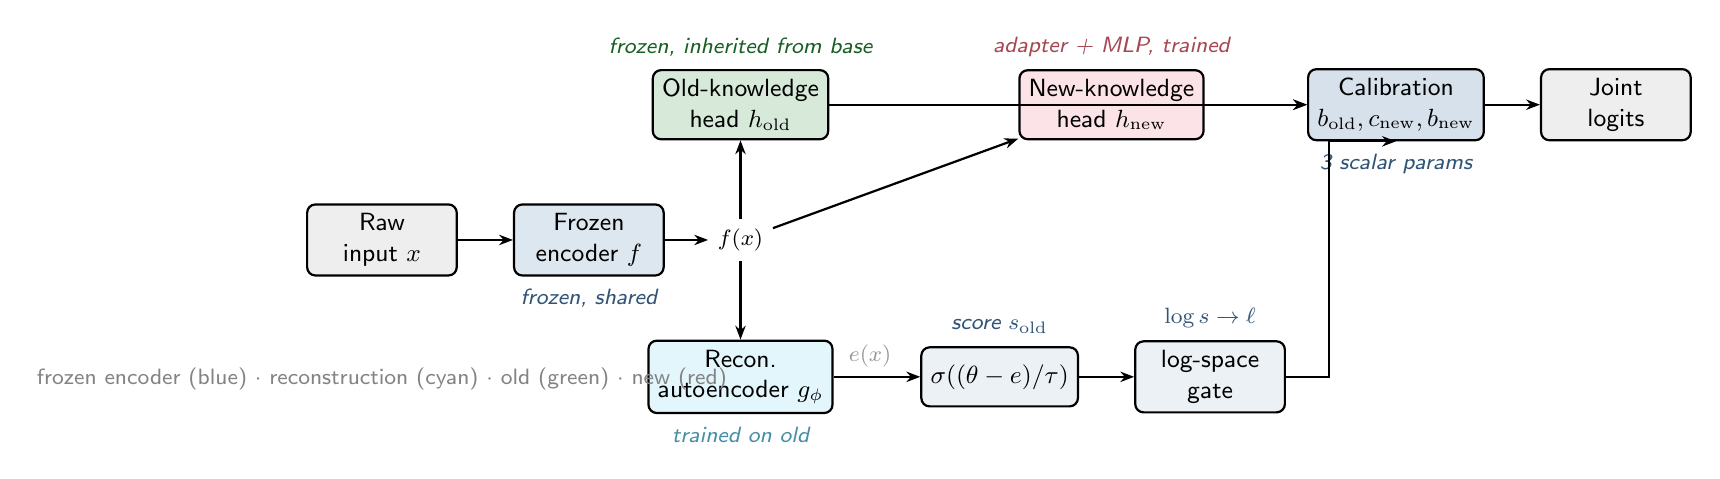
\begin{tikzpicture}[
    node distance=0.55cm and 0.7cm,
    box/.style={rectangle, draw, thick, rounded corners=3pt,
                minimum width=1.9cm, minimum height=0.75cm,
                font=\small\sffamily, align=center},
    raw/.style={box, fill=ptgrey!25},
    enc/.style={box, fill=ptblue!18},
    ae/.style={box, fill=ptcyan!18},
    prob/.style={box, fill=ptblue!10},
    hold/.style={box, fill=ptgreen!18},
    hnew/.style={box, fill=ptred!18},
    calib/.style={box, fill=ptblue!22},
    small/.style={font=\footnotesize\sffamily},
    smallit/.style={font=\footnotesize\sffamily\itshape},
    arrow/.style={-{Stealth[length=5pt]}, thick},
    arrowthin/.style={-{Stealth[length=4pt]}, thick, color=ptgrey},
]

% --- input ---
\node[raw] (in) {Raw\\input $x$};

% --- frozen encoder ---
\node[enc, right=of in] (enc) {Frozen\\encoder $f$};
\node[smallit, below=1pt of enc, color=ptblue!70!black] {frozen, shared};

% --- feature (fork point) ---
\node[small, right=0.55cm of enc] (feat) {$f(x)$};

% --- autoencoder branch (drops down then up) ---
\node[ae, below=1.0cm of feat] (ae) {Recon.\\autoencoder $g_\phi$};
\node[smallit, below=1pt of ae, color=ptcyan!70!black] {trained on old};

% --- sigmoid + threshold/tau ---
\node[prob, right=1.1cm of ae] (sig) {$\sigma((\theta - e)/\tau)$};
\node[prob, right=of sig] (gate) {log-space\\gate};
\node[smallit, above=1pt of sig, color=ptblue!70!black] {score $s_{\mathrm{old}}$};
\node[smallit, above=1pt of gate, color=ptblue!70!black] {$\log s \to \ell$};

% --- two heads ---
\node[hold, above=1.0cm of feat] (hold) {Old-knowledge\\head $h_{\mathrm{old}}$};
\node[smallit, above=1pt of hold, color=ptgreen!70!black] {frozen, inherited from base};
\node[hnew, right=2.4cm of hold] (hnew) {New-knowledge\\head $h_{\mathrm{new}}$};
\node[smallit, above=1pt of hnew, color=ptred!70!black] {adapter + MLP, trained};

% --- calibration ---
\node[calib, right=1.3cm of hnew] (calib) {Calibration\\$b_{\mathrm{old}}, c_{\mathrm{new}}, b_{\mathrm{new}}$};
\node[smallit, below=1pt of calib, color=ptblue!70!black] {3 scalar params};

% --- output ---
\node[raw, right=of calib] (out) {Joint\\logits};

% ============== arrows ==============
\draw[arrow] (in) -- (enc);
\draw[arrow] (enc) -- (feat);

% feature -> heads (fan-out)
\draw[arrow] (feat) -- (hold);
\draw[arrow] (feat) -- (hnew);

% feature -> autoencoder (down)
\draw[arrow] (feat) -- (ae);
% autoencoder -> sigmoid -> gate
\draw[arrow] (ae) -- (sig);
\draw[arrow] (sig) -- (gate);

% gate -> calibration (log-space routing signal feeds into combination)
\draw[arrow] (gate.east) -- ++(0.55cm,0) |- (calib.south);

% heads -> calibration
\draw[arrow] (hold) -- (calib);
\draw[arrow] (hnew) -- (calib);

% calibration -> output
\draw[arrow] (calib) -- (out);

% --- error term annotation ---
\node[small, color=ptgrey!80!black, above] at ($(ae)!0.5!(sig)$) {$e(x)$};

% --- legend hint ---
\node[small, color=ptgrey!70!black] at ($(in.south)+(0,-1.3cm)$)
    {frozen encoder (blue) $\cdot$ reconstruction (cyan) $\cdot$ old (green) $\cdot$ new (red)};

\end{tikzpicture}

\caption{RAR architecture overview.}
\label{fig:rar-architecture}
\Description{Architecture diagram of RAR. Each flow passes through a frozen ET-BERT encoder into feature vector f(x). Three parallel branches contain a frozen old-class path, a trainable new-class path with an adapter, and a reconstruction autoencoder that maps error through a sigmoid into routing scores. Log-space gating combines the two class-path outputs, followed by scalar calibration into joint logits.}
\end{figure*}

% -----------------------------------------------------------------
% 3.1 Problem formulation
% -----------------------------------------------------------------
\subsection{Problem Formulation}

Let $f: \mathcal{X} \to \mathbb{R}^d$ be a frozen encoder pre-trained on large-scale encrypted traffic data (ET-BERT~\cite{lin2022etbert}). At the base stage, we train a classifier $F_0$ on $K_0$ classes using $\mathcal{D}_0 = \{(x_i,y_i)\}_{i=1}^{N_0}$. At increment $t$, $K_t$ classes arrive with data $\mathcal{D}_t$, and a replay buffer $\mathcal{B}_{t-1}$ represents the classes seen before $t$. Let $K_{<t}=\sum_{j=0}^{t-1}K_j$ denote the number of previously learned classes. RAR freezes the complete preceding classifier $F_{t-1}$ as the old prediction path and learns a new-class head $h_t:\mathbb{R}^d\to\mathbb{R}^{K_t}$. For the single-increment setting, $F_{t-1}=F_0$ reduces to the frozen base classifier. Each flow is routed between $F_{t-1}$ and $h_t$ by a weight derived from reconstruction error. The following subsections define the reconstruction signal (\S\ref{sec:knowledge}), routing (\S\ref{sec:routing}), calibration (\S\ref{sec:calib}), and training procedure (\S\ref{sec:training}).

% -----------------------------------------------------------------
% 3.2 Per-flow reconstruction compatibility
% -----------------------------------------------------------------
\subsection{Per-Flow Reconstruction Compatibility}\label{sec:knowledge}

% Topic sentence 1: claim
RAR measures each flow's compatibility with the replay-derived historical-class manifold using a scalar routing score. This score is an operational weight, not a calibrated posterior probability or a hard assignment to one class group.

% Topic sentence 2: mechanism
We train a reconstruction autoencoder $g_\phi$ on frozen-encoder features of replayed old samples, so $g_\phi$ learns the manifold that the frozen encoder $f$ produces for old classes. The reconstruction error therefore tends to be small on old-class samples and large on new-class samples:
\begin{equation}\label{eq:recon}
e(x) = \frac{1}{d}\,\| g_\phi(f(x)) - f(x) \|_2^2.
\end{equation}
We compute the old 95th-percentile edge and new 5th-percentile edge on the replay and new reference sets, respectively, and set $\theta$ to their midpoint. The temperature $\tau$ is the pooled standard deviation of their errors, lower-bounded for numerical stability. We then convert the error to per-flow routing scores:
\begin{align}
s_{\mathrm{old}}(x) &= \sigma\!\left(\frac{\theta - e(x)}{\tau}\right),\label{eq:score-old}\\
s_{\mathrm{new}}(x) &= 1 - s_{\mathrm{old}}(x),\label{eq:score-new}
\end{align}
where $\tau$ controls the sharpness of the sigmoid. The fitted threshold and temperature are fixed after the pre-training stage; only $e(x)$ is computed per input at inference.

% Topic sentence 3: why reconstruction (design justification)
The score does not require a class label at inference: it measures compatibility between $f(x)$ and the feature manifold learned by $g_\phi$. Its fitting stage does use the known old/new split between replay and newly arriving reference samples. Reconstruction-based gating has previously been used to infer tasks and select experts~\cite{aljundi2017expertgate}; here, the score instead balances two class groups within a unified prediction space and weights the corresponding incremental-learning objectives. It complements output-based distillation (LwF~\cite{li2017lwf}, iCaRL~\cite{rebuffi2017icarl}) and stored-example replay (DER~\cite{yan2021der}).

% Topic sentence 4: empirical foundation
The empirical foundation for $s_{\mathrm{old}}$ is separability: across the six evaluated datasets, reconstruction error distinguishes old from new samples with mean AUC 0.894 (Figure~\ref{fig:e0-separability}). This result motivates evaluating the routing mechanism on the full benchmark; it does not imply perfect old/new identification.

\begin{figure*}[t]
\centering
% =============================================================
% RAR -- Figure 2: Reconstruction routing mechanism (detail)
% Label: fig:recon-routing
% Used in: Per-Flow Reconstruction Compatibility.
% Format: input-style (no \documentclass). \input{} from paper.tex.
%   For standalone visual preview, wrap in
%     \documentclass[border=5pt]{standalone}
%     \usepackage{tikz} \usetikzlibrary{...}
%     \definecolor{ptblue}{HTML}{4477AA} ... (palette)
% Color palette: Paul Tol bright (matches figures/fig_*.tex).
% =============================================================

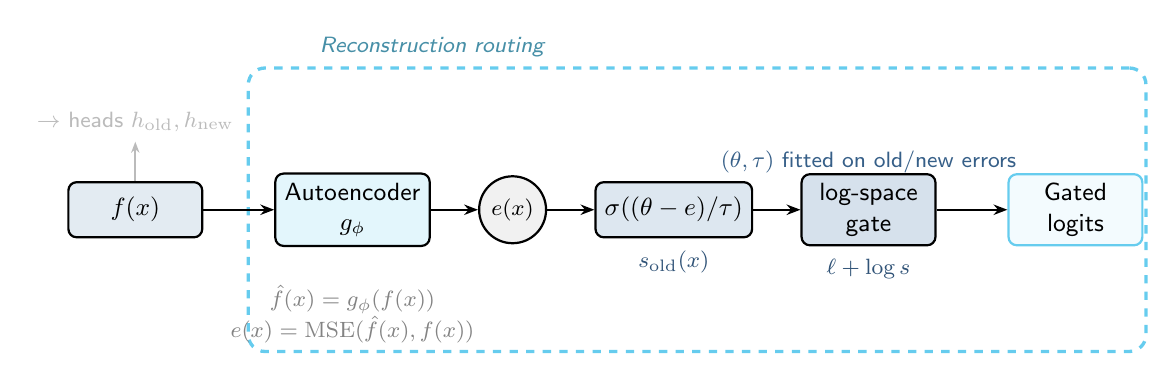
\begin{tikzpicture}[
    node distance=0.6cm and 0.6cm,
    box/.style={rectangle, draw, thick, rounded corners=3pt,
                minimum width=1.7cm, minimum height=0.7cm,
                font=\small\sffamily, align=center},
    fbox/.style={box, fill=ptblue!15},
    ae/.style={box, fill=ptcyan!18},
    err/.style={circle, draw, thick, fill=ptgrey!20,
                minimum size=0.85cm, inner sep=1pt,
                font=\footnotesize\sffamily},
    sigbox/.style={box, fill=ptblue!18},
    taubox/.style={box, fill=ptblue!22},
    small/.style={font=\footnotesize\sffamily},
    smallit/.style={font=\footnotesize\sffamily\itshape},
    arrow/.style={-{Stealth[length=5pt]}, thick},
    arrowthin/.style={-{Stealth[length=4pt]}, thick, color=ptgrey},
]

% --- bounding dashed box (drawn first; nodes will sit on top) ---
\node[draw=ptcyan, very thick, dashed, rounded corners=6pt,
      minimum width=11.4cm, minimum height=3.6cm,
      label={[smallit, color=ptcyan!70!black]above left:Reconstruction routing}] (bound) {};

% --- feature input ---
\node[fbox, left=0.55cm of bound.west, anchor=east] (feat) {$f(x)$};

% --- autoencoder ---
\node[ae, right=0.9cm of feat] (ae) {Autoencoder\\$g_\phi$};

% --- error ---
\node[err, right=of ae] (err) {$e(x)$};

% --- sigmoid with fitted threshold + temperature ---
\node[sigbox, right=of err] (sig) {$\sigma((\theta - e) / \tau)$};
\node[smallit, below=1pt of sig, color=ptblue!70!black]
    {$s_{\mathrm{old}}(x)$};

% --- log-space gating ---
\node[taubox, right=of sig] (tau) {log-space\\gate};
\node[smallit, below=1pt of tau, color=ptblue!70!black]
    {$\ell + \log s$};

% --- output ---
\node[box, draw=ptcyan, thick, fill=ptcyan!8,
      right=0.9cm of tau] (out) {Gated\\logits};

% ============== arrows ==============
\draw[arrow] (feat) -- (ae);
\draw[arrow] (ae) -- (err);
\draw[arrow] (err) -- (sig);
\draw[arrow] (sig) -- (tau);
\draw[arrow] (tau) -- (out);

% --- external thin arrows showing f(x) also goes to heads ---
\draw[arrowthin] (feat.north) -- ++(0,0.5cm) node[above, small, color=ptgrey]
    {$\to$ heads $h_{\mathrm{old}}, h_{\mathrm{new}}$};

% --- tau + theta annotation ---
\node[small, color=ptblue!80!black, above=4pt of tau.north, anchor=center]
    {$(\theta, \tau)$ fitted on old/new errors};

% --- eqn under sigmoid ---
\node[small, color=ptgrey!70!black, align=center]
    at ($(ae.south)+(0,-0.85cm)$)
    {$\hat f(x) = g_\phi(f(x))$\\$e(x) = \mathrm{MSE}(\hat f(x), f(x))$};

\end{tikzpicture}

\caption{Reconstruction routing mechanism.}
\label{fig:recon-routing}
\Description{Detailed view of the reconstruction routing mechanism. Frozen encoder features pass through a feature reconstructor, producing reconstruction error via mean squared error. A fitted threshold and temperature map the error through a sigmoid into an old-sample score. The score is applied as an additive log-space gate to the dual-head logits before concatenation and calibration.}
\end{figure*}

\begin{figure}[t]
\centering
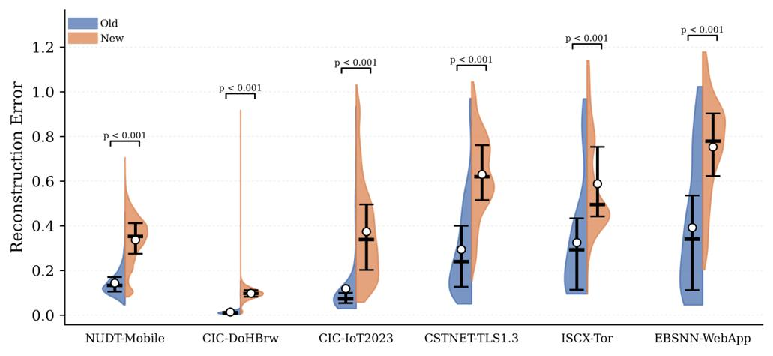
\includegraphics[width=\linewidth]{figures/fig_e0_separability.pdf}
\caption{Per-dataset reconstruction-error distributions (old vs.\ new).}
\label{fig:e0-separability}
\Description{Six-panel violin plot showing per-dataset distributions of reconstruction error for old and new samples. Blue violins represent old-class errors, orange violins represent new-class errors. All six datasets show statistically significant separation (p less than 0.001). Datasets: NUDT-Mobile, CIC-DoHBrw, CIC-IoT2023, CSTNET-TLS1.3, ISCX-Tor, EBSNN-WebApp.}
\end{figure}

% -----------------------------------------------------------------
% 3.3 Soft routing and dual class paths
% -----------------------------------------------------------------
\subsection{Soft Routing and Dual Class Paths}\label{sec:routing}

% Topic sentence 1: claim
RAR routes each flow through two class paths: the frozen preceding classifier $F_{t-1}$ and a trainable new-class head $h_t$ equipped with a lightweight adapter. Their outputs are weighted by $s_{\mathrm{old}}(x)$ and $s_{\mathrm{new}}(x)$ from Eqs.~\eqref{eq:score-old}--\eqref{eq:score-new}.

% Topic sentence 2: what each head does
In the first increment, the old path is the frozen base-stage classifier. In later increments, it is the complete recursively constructed RAR classifier from the preceding step and therefore covers all previously seen classes. The current new head is trained through a residual adapter and a LayerNorm+MLP pathway. The current encoder remains frozen.

% Topic sentence 3: soft routing mechanism
We apply the routing signal in log space. Let $\ell_{\mathrm{old}}(x) \in \mathbb{R}^{K_{<t}}$ and $\ell_{\mathrm{new}}(x) \in \mathbb{R}^{K_t}$ be the raw logit vectors from the two paths. The gated logits are computed by adding the log of each path's routing score:
\begin{align}
\tilde{\ell}_{\mathrm{old}}(x) &= \ell_{\mathrm{old}}(x) + \log s_{\mathrm{old}}(x),\label{eq:routing-old}\\
\tilde{\ell}_{\mathrm{new}}(x) &= \ell_{\mathrm{new}}(x) + \log s_{\mathrm{new}}(x).\label{eq:routing-new}
\end{align}
The two gated vectors are concatenated into a joint prediction over all $K_{<t} + K_t$ classes:
\begin{equation}\label{eq:concat}
\hat{y} = \mathrm{softmax}\bigl([\,\tilde{\ell}_{\mathrm{old}}(x)\;;\;\tilde{\ell}_{\mathrm{new}}(x)\,]\bigr).
\end{equation}
In softmax space, adding $\log s$ is equivalent to multiplying the head's class probabilities by $s$: the old-head probabilities are scaled by $s_{\mathrm{old}}(x)$ and the new-head probabilities by $s_{\mathrm{new}}(x)$, so both heads contribute to every prediction according to the flow's historical-class compatibility. As $\tau \to 0$ the sigmoid sharpens toward a step function and $s_{\mathrm{old}}$ approaches $0$ or $1$; as $\tau \to \infty$ the sigmoid flattens and both heads contribute near-equally. \S\ref{sec:eval-ablation-tau} reports the empirical trade-off.

% Topic sentence 4: why dual heads (design justification)
We separate old and new paths because standard head expansion makes their logits compete within one trainable decision space~\cite{rebuffi2017icarl,wu2019bic}. Under imbalanced replay, optimization can favor the newly arriving group. Freezing the preceding path prevents direct updates to its class-specific parameters, while the calibration step makes its logits comparable with those of the new head. Table~\ref{tab:ablation} measures the contribution of this separation.

% Topic sentence 5: soft vs hard
We use soft routing because hard assignment routes every sample to a single head and discards the second head's view entirely. On samples near the reconstruction-error decision boundary, the discarded head often holds the correct prediction. Soft routing keeps both views available and shifts their contribution with the input, so the calibration step is structurally necessary: the two heads cannot be averaged directly because they output logits over disjoint class subsets.

% -----------------------------------------------------------------
% 3.3 Logit calibration 
% -----------------------------------------------------------------
\subsection{Logit Calibration}\label{sec:calib}

% Topic sentence 1: claim
Each head outputs logits over its own class subset; a calibration layer removes the scale mismatch between the two paths before their logits are combined.

% Topic sentence 2: why calibration is needed
The two heads live on different class axes and may produce logits at different magnitudes. A naive concatenation would let the head with larger logits dominate Eq.~\eqref{eq:concat} regardless of the routing scores. Calibration equalizes the two heads' output scales on a held-out validation set before the logits are combined.

% Topic sentence 3: calibration mechanism
We learn three scalar parameters: a subtractive bias $b_{\mathrm{old}} \in \mathbb{R}$ on the old-path logits, a multiplicative scale $c_{\mathrm{new}} \in \mathbb{R}^+$, and an additive bias $b_{\mathrm{new}} \in \mathbb{R}$ on the new-head logits:
\begin{align}
\ell'_{\mathrm{old}} &= \tilde{\ell}_{\mathrm{old}} - b_{\mathrm{old}},\label{eq:calib-old}\\
\ell'_{\mathrm{new}} &= c_{\mathrm{new}} \cdot \tilde{\ell}_{\mathrm{new}} + b_{\mathrm{new}},\label{eq:calib-new}
\end{align}
where $\tilde{\ell}_{\mathrm{old}}, \tilde{\ell}_{\mathrm{new}}$ are the gated logits from Eqs.~\eqref{eq:routing-old}--\eqref{eq:routing-new}. The concatenation in Eq.~\eqref{eq:concat} then uses $[\ell'_{\mathrm{old}}; \ell'_{\mathrm{new}}]$. The three scalars are optimized with the new-class pathway during incremental training and then refined, with both prediction paths frozen, on a balanced calibration set formed from replayed old samples and held-out new samples.

% Topic sentence 4: what calibration does and does not do
Calibration does not change which classes the paths cover; it only adjusts their relative output scales. The classification decision remains a weighted combination in which the weights come from the reconstruction-derived routing score. Table~\ref{tab:ablation} reports its contribution.

% -----------------------------------------------------------------
% 3.4 Training objective and the temperature tau knob 
% -----------------------------------------------------------------
\subsection{Training Objective}\label{sec:training}

RAR training proceeds in three phases at each increment.

\paragraph{Phase 1: Fitting the reconstructor.}
We fit the reconstruction autoencoder $g_\phi$ on frozen-encoder features of replayed old samples by minimizing $\mathcal{L}_{\mathrm{recon}} = \frac{1}{|\mathcal{B}|}\sum_{x \in \mathcal{B}} \|g_\phi(f(x)) - f(x)\|_2^2$. We then estimate $\theta$ and $\tau$ from replayed-old and held-out-new errors as described in \S\ref{sec:knowledge}, and freeze $g_\phi$.

\paragraph{Phase 2: Incremental training.}
We freeze the preceding prediction path and optimize the adapter, new-class pathway, and calibration scalars with the following composite loss:
\begin{align}
\mathcal{L} &= \mathcal{L}_{\mathrm{CE}} + \alpha \mathcal{L}_{\mathrm{distill}} + \beta \mathcal{L}_{\mathrm{local}} + \gamma \mathcal{L}_{\mathrm{margin}} + \delta \mathcal{L}_{\mathrm{reg}},\label{eq:loss}\\[2pt]
\mathcal{L}_{\mathrm{distill}} &= \frac{1}{Z}\sum_{x \in \mathcal{B}} s_{\mathrm{old}}(x)\, D_{\mathrm{KL}}\bigl(F_{t-1}(x) \;\big\|\; \ell_{\mathrm{old}}(x)\bigr).\label{eq:distill}
\end{align}
Here $\ell_{\mathrm{old}}$ denotes the preceding path's logits after the trainable old-path bias, so the KL term anchors this adjustment to the frozen teacher output; the class-specific parameters of $F_{t-1}$ remain frozen. $\mathcal{L}_{\mathrm{CE}}$ is cross-entropy on the concatenated output over all classes; $\mathcal{L}_{\mathrm{local}}$ is cross-entropy restricted to the new head on new-class samples; $\mathcal{L}_{\mathrm{margin}}$ penalizes the old path for outscoring the correct new-class logit, weighted by $s_{\mathrm{new}}(x)$; and $\mathcal{L}_{\mathrm{reg}} = \|a(x) - f(x)\|_2^2$ regularizes the adapter shift from the frozen features. The replay buffer uses 1\% of the old training data in the main comparison; \S\ref{sec:eval-buffer} sweeps this ratio.

\paragraph{Phase 3: Calibration refinement.}
After incremental training, we freeze both prediction paths and refine $(b_{\mathrm{old}}, c_{\mathrm{new}}, b_{\mathrm{new}})$ on a balanced mixed calibration set by minimizing cross-entropy. The old portion is sampled from replay memory; the new portion comes from a fixed new-class validation partition that is excluded from final testing.

\subsection{Recursive Multi-step Update}\label{sec:multistep}
For sequential increments, RAR applies the same construction recursively. After increment $t$, the complete calibrated classifier $F_t$, including its earlier routing hierarchy, is frozen and used as the old path at increment $t+1$. The replay buffer is resampled from all classes seen through $t$, and a fresh reconstructor, threshold, temperature, adapter, and new-class head are fitted for the next class block. Consequently, the old output dimension grows from $\sum_{j=0}^{t-1}K_j$ to $\sum_{j=0}^{t}K_j$ without flattening the previous heads into a newly trainable shared classifier. This is the protocol used in the five-increment experiment in \S\ref{sec:eval-buffer}.

\paragraph{Algorithm.}
Algorithm~\ref{alg:rar} summarizes the full training and inference procedure.

\begin{algorithm}[t]
\SetAlgoNoLine
\KwIn{Frozen preceding classifier $F_{t-1}$; replay buffer $\mathcal{B}_{t-1}$; current data $\mathcal{D}_t$; reconstructor $g_\phi$; temperature $\tau$}
\KwOut{Incremental classifier $F$}
\For{each batch from $\mathcal{B} \cup \mathcal{D}_{\mathrm{new}}$}{
  \textbf{Feature extraction}\;
  \Indp
  $z \gets f(x)$ \quad (frozen, no gradient)\;
  \Indm
  \textbf{Reconstruction error}\;
  \Indp
  $e(x) = \frac{1}{d}\,\|g_\phi(z)-z\|_2^2$\;
  \Indm
  \textbf{Old/new routing score}\;
  \Indp
  $s_{\mathrm{old}}
  = \sigma\!\left(\frac{\theta-e(x)}{\tau}\right)$\;
  $s_{\mathrm{new}}
  = 1-s_{\mathrm{old}}$\;
  \Indm
  \textbf{Dual-head routing (log-space)}\;
  \Indp
  $\tilde{\ell}_{\mathrm{old}}
  = \ell_{\mathrm{old}}
  +\log s_{\mathrm{old}}$\;

  $\tilde{\ell}_{\mathrm{new}}
  = \ell_{\mathrm{new}}
  +\log s_{\mathrm{new}}$\;

  $\hat{y}
  =\mathrm{softmax}
  ([\tilde{\ell}_{\mathrm{old}};
  \tilde{\ell}_{\mathrm{new}}])$\;
  \Indm

  \textbf{Training objective}\;
  \Indp
  $\mathcal{L}
  =
  \mathcal{L}_{\mathrm{CE}}
  +\alpha\mathcal{L}_{\mathrm{distill}}
  +\beta\mathcal{L}_{\mathrm{local}}
  +\gamma\mathcal{L}_{\mathrm{margin}}
  +\delta\mathcal{L}_{\mathrm{reg}}$\;
  \Indm
}
\textbf{Post-hoc calibration}\;
\Indp
$\ell'_{\mathrm{old}}
=\tilde{\ell}_{\mathrm{old}}-b_{\mathrm{old}}$\;

$\ell'_{\mathrm{new}}
=c_{\mathrm{new}}\cdot\tilde{\ell}_{\mathrm{new}}+b_{\mathrm{new}}$\;

Refine $(b_{\mathrm{old}}, c_{\mathrm{new}}, b_{\mathrm{new}})$ on the mixed calibration set (paths frozen)\;
\Indm
\Return $F$
\caption{Reconstruction-Aware Routing (RAR)}
\label{alg:rar}
\end{algorithm}

% Topic sentence 5: the tau knob
The temperature $\tau$ trades routing determinism against path fusion. In the implementation it is estimated from the pooled reconstruction-error spread; \S\ref{sec:eval-ablation-tau} additionally reports a controlled sensitivity sweep. Lowering $\tau$ makes the routing weights more discrete, but does not by itself reduce computation because both paths are still evaluated.

% -----------------------------------------------------------------
% 3.5 Assumptions and failure modes 
% -----------------------------------------------------------------
\subsection{Applicability and Assumptions}\label{sec:assumptions}

RAR is designed under two key assumptions that define its applicability.

First, replay memory should provide representative coverage of previously learned classes. If replay samples fail to capture the historical-class distribution, the reconstructor may learn an incomplete historical manifold, leading to inaccurate routing scores. \S\ref{sec:eval-buffer} evaluates different replay buffer sizes and shows that RAR remains robust even under a memory ratio of 0.005.

Second, reconstruction error should exhibit sufficient separability between old and emerging knowledge. When old and new classes have highly similar feature representations, reconstruction errors may overlap, reducing the reliability of the compatibility score. Figure~\ref{fig:e0-separability} shows the observed separation across the six evaluated datasets.

These assumptions characterize the applicability of RAR rather than strict limitations. RAR is most effective when replay samples preserve representative historical-class coverage and when old and emerging classes exhibit distinguishable representation patterns.

% !TEX root = paper.tex
% =============================================================
% RAR — Evaluation Section Scaffold (v0)
% Source-of-truth: project_context.md (Binding constraints).
% Stage 3 of paper-writing skill. Draft 0 intro frozen 2026-07-09.
% Last updated: 2026-07-09
%
% Conventions
%   - KDD venue: integrated related work, colon-style subtitles, no \smartparagraph.
%   - Headings are claims. Topic sentences assert claims.
%   - Every subsection ends with a "Takeaway." paragraph.
%   - Main tables have been populated from the organized results.
%   - Reference metadata remains to be finalized before submission.
%   - Mechanism: SOFT routing via reconstruction-temperature-weighted dual heads.
%     Do not describe RAR as assigning each sample to a single head.
% =============================================================

\section{Experiments}\label{sec:eval}
% Section opener: claim-first. The headline number lives in the section heading.
% Each subsection below tests a specific claim from the introduction (C1--C4).
% Setup first (§4.1), then head-to-head (§4.2 and §4.3 split by Principle 9),
% then ablations (§4.4), optional robustness (§4.5), then honest disaggregation (§4.6).

% -----------------------------------------------------------------
% §4.1 Setup Anchoring  -- full prose per the deferred-action contract
% -----------------------------------------------------------------
\subsection{Experimental Setup}

We evaluate RAR on six public encrypted-traffic datasets that span several application and threat surfaces: mobile app traffic (NUDT-Mobile), DNS-over-HTTPS (CIC-DoHBrw), IoT attack traffic (CIC-IoT2023), TLS~1.3 application traffic (CSTNET-TLS1.3), Tor traffic (ISCX-Tor), and web application traffic (EBSNN-WebApp). Table~\ref{tab:datasets} reports their sizes and class counts.

\begin{table}[t]
\caption{Six encrypted-traffic datasets used in evaluation.}
\label{tab:datasets}
\centering
\footnotesize
\begin{tabular}{p{2.4cm}llrr}
\toprule
Dataset & Domain & Public & \#Cls & \#Flows \\
\midrule
NUDT-Mobile      & Mobile app     & Yes & 300 & 496086 \\
CIC-DoHBrw       & DNS-over-HTTPS & Yes & 6 & 49777 \\
CIC-IoT2023      & IoT attack     & Yes & 22 & 26413 \\
CSTNET-TLS1.3    & TLS 1.3 app    & Yes & 120 & 43243 \\
ISCX-Tor         & Tor            & Yes & 26 & 8518 \\
EBSNN-WebApp     & Web app        & Yes & 48 & 15336 \\
\bottomrule
\end{tabular}
\end{table}

We compare RAR against two baseline groups. \emph{Group A} holds the encoder fixed at ET-BERT~\cite{lin2022etbert} and varies the CIL strategy: Learning without Forgetting (LwF)~\cite{li2017lwf}, iCaRL~\cite{rebuffi2017icarl}, BiC~\cite{wu2019bic}, DER~\cite{yan2021der}, Adapter~\cite{houlsby2019adapter}, Fine-tune, and an ET-BERT adaptation of MORE~\cite{kim2022more}. \emph{Group B} holds the naive CIL setup fixed and varies the traffic-classification backbone across nine models: AppScanner, ETC-PS, FlowLens, CNN-based, CNN-emb, EBSNN, FS-Net, GraphDApp, and MM4flow. RAR with ET-BERT is included as a reference rather than counted as a tenth backbone baseline. Group~A compares routing with both classical CIL strategies and a closely related OOD-replay multi-head method on a fixed encoder; Group~B tests whether naive incremental forgetting persists across encoder choices.

\begin{table}[t]
\caption{Baseline groups.}
\label{tab:baselines}
\centering
\small
\begin{tabular}{lll}
\toprule
Group & Variable held fixed & Baselines \\
\midrule
A & ET-BERT encoder & LwF, iCaRL, BiC, DER, Adapter,\\
  &                   & Fine-tune, MORE \\
B & Replay + head expansion & AppScanner, ETC-PS, FlowLens,\\
  &                        & CNN-based, CNN-emb, EBSNN,\\
  &                        & FS-Net, GraphDApp, MM4flow \\
\bottomrule
\end{tabular}
\end{table}

Five metrics isolate the quantity each claim depends on. \emph{old-before} measures accuracy on old classes after head expansion and \emph{before} training on the new step. \emph{old-after} measures accuracy on old classes after training on the new step. \emph{new-after-train} measures accuracy on the new classes after the new step. \emph{mix} reports combined accuracy on old plus new classes after the new step. \emph{forgetting} equals \emph{old-before} minus \emph{old-after} and isolates training-induced forgetting, so the head-expansion drop alone does not contribute.

We report forgetting and mix as the headline pair: forgetting measures old-class retention after incremental training, and mix captures the joint old/new accuracy that operators observe. Together they evaluate the two outcomes that reconstruction-conditioned balancing is designed to improve.

All experiments share one training and evaluation pipeline. The encoder remains frozen. During an increment, the inherited old path and the fitted reconstructor are frozen; the adapter, new-class pathway, and calibration scalars are trainable. The calibration scalars are subsequently refined on a mixed validation set.

Before incremental training, we repartition the provided new-class evaluation split using a fixed random seed (42), reserving 10\% for validation and the remaining 90\% for held-out testing. The validation and held-out test subsets are disjoint, and the old-class test split is evaluated independently.

The main comparison uses a two-stage protocol: a base stage trains the initial head on the first half of classes, and one incremental stage learns the remaining classes with a fixed replay buffer. Section~\ref{sec:eval-buffer} additionally evaluates the recursive five-increment protocol defined in Section~\ref{sec:multistep}.

% -----------------------------------------------------------------
% §4.2 Group A -- RAR vs classical CIL strategies. Topic sentences + table + Takeaway.
% -----------------------------------------------------------------
\subsection{Comparison with CIL Strategies}
% Tests C1: reconstruction-aware old/new balancing.
% Headline: forgetting cut by 35.5%--67.5% (vs Adapter, mean 47.8%); mix raised by up to 11.7 pp.

% Topic sentence 1: claim
Against classical CIL strategies on a fixed ET-BERT encoder, RAR cuts forgetting by an average of 47.8\% (range 35.5\%--67.5\%) across six datasets and raises mixed-class accuracy by up to 11.7 percentage points over the strongest evaluated baseline (Adapter).

% Topic sentence 2: pattern
Replay-based methods (DER, iCaRL) outperform uniform distillation (LwF) under encrypted traffic, yet both still forget more than RAR on every dataset.

% Topic sentence 3: fine-tuning reference
Fine-tune, which omits all anti-forgetting mechanisms, provides a naive incremental reference. RAR reduces forgetting by 35.5\%--67.5\% relative to the strongest evaluated baseline (Adapter) on every dataset.

% Topic sentence 4: pattern citation (Principle 14)
The consistent gains are compatible with the intended effect of reconstruction-error routing: adapting preservation and acquisition signals to each flow rather than applying a uniform balance.

% Topic sentence 5: figure/table reference
\begin{table*}[t]
\caption{Forgetting ($F\!\downarrow$, lower is better) and mixed-class accuracy ($M\!\uparrow$, higher is better). Mean over 3 seeds; \emph{TBD} marks runs in progress.}
\label{tab:eval-a}
\centering
\small
\setlength{\tabcolsep}{6pt}
\renewcommand{\arraystretch}{1.05}

\begin{tabular}{p{1.8cm}|
>{\centering\arraybackslash}p{0.55cm}@{\hspace{8pt}}
>{\centering\arraybackslash}p{0.55cm}|
>{\centering\arraybackslash}p{0.55cm}@{\hspace{8pt}}
>{\centering\arraybackslash}p{0.55cm}|
>{\centering\arraybackslash}p{0.55cm}@{\hspace{8pt}}
>{\centering\arraybackslash}p{0.55cm}|
>{\centering\arraybackslash}p{0.55cm}@{\hspace{8pt}}
>{\centering\arraybackslash}p{0.55cm}|
>{\centering\arraybackslash}p{0.55cm}@{\hspace{8pt}}
>{\centering\arraybackslash}p{0.55cm}|
>{\centering\arraybackslash}p{0.55cm}@{\hspace{8pt}}
>{\centering\arraybackslash}p{0.55cm}
}
\toprule

& \multicolumn{12}{c}{Dataset} \\
\cmidrule(lr){2-13}
Method
& \multicolumn{2}{c|}{NUDT}
& \multicolumn{2}{c|}{DoH}
& \multicolumn{2}{c|}{IoT}
& \multicolumn{2}{c|}{TLS}
& \multicolumn{2}{c|}{Tor}
& \multicolumn{2}{c}{Web} \\

& $F\!\downarrow$
& $M\!\uparrow$
& $F\!\downarrow$
& $M\!\uparrow$
& $F\!\downarrow$
& $M\!\uparrow$
& $F\!\downarrow$
& $M\!\uparrow$
& $F\!\downarrow$
& $M\!\uparrow$
& $F\!\downarrow$
& $M\!\uparrow$ \\

\midrule
Fine-tune & 95.40 & 33.71 & 91.58 & 36.74 & 88.52 & 11.17 & 90.99 & 46.52 & 86.25 & 41.31 & 86.01 & 43.19 \\
LwF~\cite{li2017lwf} & 61.03 & 55.91 & 88.91 & 36.75 & 52.58 & 43.53 & 56.21 & 65.66 & 96.37 & 34.72 & 78.11 & 48.20 \\
iCaRL~\cite{rebuffi2017icarl} & 25.15 & 81.66 & 33.87 & 73.25 & 12.39 & 79.47 & 28.87 & 80.83 & 73.60 & 69.90 & 37.77 & 73.97 \\
BiC~\cite{wu2019bic} & 24.78 & 79.48 & 33.87 & 73.25 & 11.68 & 80.09 & 28.94 & 80.65 & 84.87 & 42.21 & 38.15 & 73.61 \\
DER~\cite{yan2021der} & 12.64 & 86.15 & 33.92 & 73.19 & 11.33 & 79.37 & 16.85 & 85.11 & 77.28 & 46.83 & 17.89 & 84.78 \\
Adapter~\cite{houlsby2019adapter} & 12.79 & 86.86 & 33.86 & 73.26 & 9.22 & 82.12 & 16.40 & 87.20 & 13.11 & 89.16 & 13.98 & 88.69 \\
MORE~\cite{kim2022more}
& \textit{TBD} & \textit{TBD}
& \textit{TBD} & \textit{TBD}
& \textit{TBD} & \textit{TBD}
& \textit{TBD} & \textit{TBD}
& \textit{TBD} & \textit{TBD}
& \textit{TBD} & \textit{TBD} \\

\midrule

RAR (ours)
& \textbf{6.65} & \textbf{90.12}
& \textbf{11.00} & \textbf{84.93}
& \textbf{4.82} & \textbf{86.05}
& \textbf{8.49} & \textbf{91.70}
& \textbf{8.45} & \textbf{91.94}
& \textbf{8.37} & \textbf{92.30} \\

\bottomrule
\end{tabular}
\end{table*}

% -----------------------------------------------------------------
% §4.3 Group B -- RAR vs 9 traffic-classification backbones.
% -----------------------------------------------------------------
\subsection{Backbone Study}\label{sec:eval-bgroup}
% Tests whether the forgetting problem depends on the encoder. Drill-down on NUDT-Mobile; Group A generalizes across the six datasets.

% Topic sentence 1: claim
On NUDT-Mobile, naive incremental training forgets across all nine traffic-classification backbones, which isolates the forgetting problem from the encoder choice.

% Topic sentence 2: pattern
Forgetting spans 13.3\%--58.4\% across the nine naive backbones despite their different representation architectures. Even the lowest-forgetting naive backbone (GraphDApp, 13.3\%) forgets more than twice as much as RAR's 6.65\% under the evaluated setup.

% Topic sentence 3: implication for encoder choice
Changing the encoder alone does not eliminate the old-class accuracy loss under naive incremental training. RAR yields lower forgetting than every naive-backbone configuration in this study (6.65\% vs 13.3\% for the lowest-forgetting configuration, GraphDApp).

% Topic sentence 4: figure/table reference
Table~\ref{tab:eval-b-forgetting} reports the naive-incremental forgetting rate and mix accuracy for each of the nine backbones on NUDT-Mobile, with RAR shown for contrast.

\begin{table}[t]
\caption{Naive-incremental forgetting and mix (\%) on NUDT-Mobile.}
\label{tab:eval-b-forgetting}
\centering
\small
\begin{tabular}{lcc}
\toprule
Backbone & Forgetting (\%) & Mix (\%) \\
\midrule
AppScanner          & 58.37 & 49.30 \\
ETC-PS              & 56.63 & 47.99 \\
FlowLens            & 56.99 & 45.69 \\
CNN-based           & 44.10 & 58.66 \\
CNN-emb             & 41.27 & 63.89 \\
EBSNN               & 30.81 & 73.37 \\
FS-Net              & 23.35 & 74.70 \\
GraphDApp           & 13.26 & 55.54 \\
MM4flow             & 22.45 & 81.61 \\
\midrule
RAR (ours)          & 6.65 & 90.12 \\
\bottomrule
\end{tabular}
\end{table}

% -----------------------------------------------------------------
% §4.4 Ablations
% -----------------------------------------------------------------
\subsection{Ablation Study}
% Tests C2, C3, and C1 attribution. E8 reports the design knob (Q28).

We ablate RAR's three principal components and its use of soft routing. \emph{w/o flow-aware routing} removes the complete per-flow reconstruction-aware routing mechanism to measure its overall contribution. \emph{w/o dual-head} replaces the old/new paths with a single expanded classifier, and \emph{w/o calibration} omits post-training logit alignment. \emph{hard routing} retains the reconstructor, dual paths, objectives, and calibration, but replaces the continuous scores with $s_{\mathrm{old}}(x)=\mathbf{1}\{e(x)\leq\theta\}$ and $s_{\mathrm{new}}(x)=1-s_{\mathrm{old}}(x)$ for binary loss weighting and single-path inference. It isolates the benefit of continuous weighting from that of flow-level old/new decisions.

\begin{table}[t]
\caption{Ablation results on NUDT-Mobile.}
\label{tab:ablation}
\centering
\small
\begin{tabular}{lcc}
\toprule
Variant & Forgetting (\%) & Mix (\%) \\
\midrule
w/o flow-aware routing & 12.43 & 87.29 \\
w/o dual-head     & 11.14 & 80.35 \\
w/o calibration   & 10.06 & 87.82 \\
hard routing      & 10.42 & 80.13 \\
\midrule
RAR (full)        & 6.65  & 90.12 \\
\bottomrule
\end{tabular}
\end{table}

Removing flow-aware routing nearly doubles forgetting, from 6.65\% to 12.43\%, demonstrating the overall effectiveness of per-flow reconstruction-aware adaptation. A single expanded head raises forgetting to 11.14\% and lowers mix from 90.12\% to 80.35\%, while removing calibration raises forgetting to 10.06\% and lowers mix to 87.82\%; these results support old/new path separation and logit alignment, respectively. Hard routing also degrades forgetting to 10.42\% and mix to 80.13\%. Its 9.99\,pp mix drop shows the cost of discarding one path after a binary decision, supporting continuous soft integration for flows near the reconstruction boundary.

% E8 -- tau sensitivity (the Q28 design knob)
\paragraph{Reconstruction temperature $\tau$ (design knob).}\label{sec:eval-ablation-tau}
Figure~\ref{fig:tau-sensitivity} reports forgetting and mix on CSTNET-TLS1.3 as $\tau$ sweeps from 0.25 (near-deterministic head selection) to 4.0 (near-uniform fusion). Forgetting drops from 9.71\% at $\tau{=}0.25$ to 7.78\% at $\tau{=}4.0$, and mix rises from 91.03\% to 92.06\%. The curve flattens after $\tau{=}1.0$: the difference between $\tau{=}1.0$ and $\tau{=}4.0$ is under 0.2\,pp on both metrics. RAR therefore exposes a tunable knob that converges quickly; the operator can fix $\tau{=}1.0$ (the fitted value) without further tuning.

\begin{figure}[t]
\centering
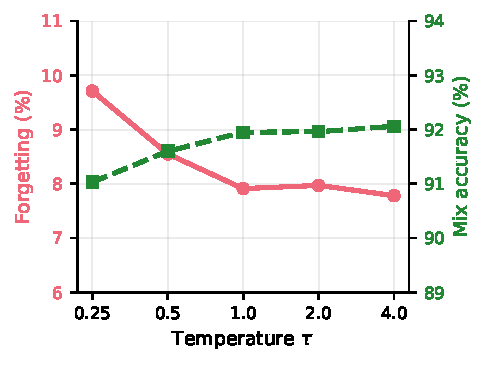
\includegraphics[width=\linewidth]{figures/tau_sensitivity.pdf}
\caption{Forgetting and mix as a function of $\tau$, on CSTNET-TLS1.3.}
\label{fig:tau-sensitivity}
\Description{Dual-axis line plot of forgetting rate and mix accuracy against temperature tau on CSTNET-TLS1.3. Red line with circles shows forgetting decreasing from 9.71 to 7.78 percent. Green dashed line with squares shows mix accuracy rising from 91.03 to 92.06 percent. The curves flatten after tau equals 1.0, indicating the sweet spot.}
\end{figure}

% -----------------------------------------------------------------
% §4.5 Robustness
% -----------------------------------------------------------------
\subsection{Robustness}\label{sec:eval-buffer}
% T = 5 steps. Buffer sweep = {5, 10, 20, 50} per class. CSTNET-TLS1.3.

% Topic sentence 1: claim
Over $T$ incremental steps and a range of replay-buffer sizes, RAR maintains its lead over Adapter, the strongest evaluated classical CIL baseline overall.

We select Adapter for these robustness experiments because it provides the strongest overall performance among the evaluated classical CIL baselines in Table~\ref{tab:eval-a}, while allowing the same frozen ET-BERT encoder, data splits, replay protocol, and memory budgets as RAR. This controlled comparison tests whether RAR's advantage persists across incremental steps and constrained replay budgets; the broader method comparison remains in Table~\ref{tab:eval-a}.

% Topic sentence 2: per-step pattern
We split the 40 new classes of CSTNET-TLS1.3 into $T=5$ steps of 8 classes each. Fine-tune collapses from 75.6\% to 22.0\% mix accuracy after five steps. Adapter degrades from 91.3\% to 74.8\%. RAR drops only from 93.4\% to 84.6\%, widening its lead over Adapter from 2.1\,pp at $T{=}1$ to 9.8\,pp at $T{=}5$.

% Topic sentence 3: buffer pattern
Across all evaluated memory ratios, RAR exhibits lower forgetting than Adapter. At the smallest ratio of 0.005, RAR records 11.82\% forgetting, compared with 22.70\% for Adapter. Increasing the ratio to 0.05 reduces the endpoint values to 5.98\% and 7.97\%, respectively, although the intermediate RAR results are not strictly monotonic. Notably, RAR at ratio 0.005 achieves forgetting comparable to Adapter at a four-times-larger ratio of 0.02 (11.82\% versus 11.70\%).

% Topic sentence 4: figure/table reference
Figure~\ref{fig:robustness} reports the per-step accuracy and buffer sensitivity on CSTNET-TLS1.3.

\begin{figure}[t]
\centering
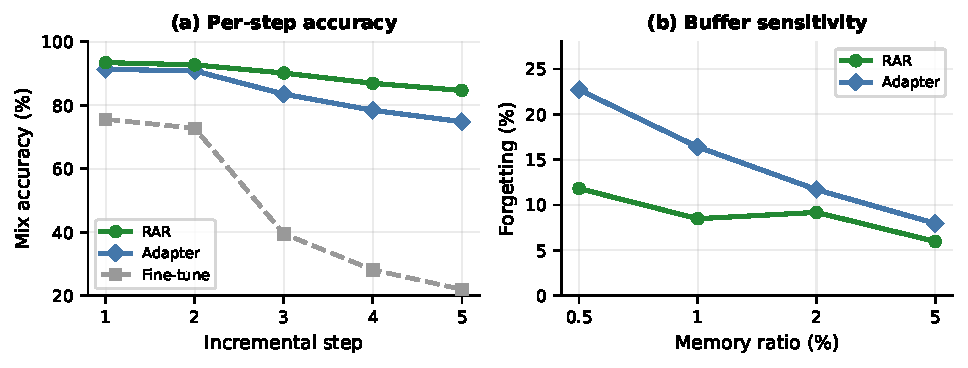
\includegraphics[width=\linewidth]{figures/robustness.pdf}
\caption{Robustness on CSTNET-TLS1.3: (a) per-step mix accuracy over $T=5$ steps, and (b) forgetting as a function of memory ratio.}
\label{fig:robustness}
\Description{Two-panel figure. Left: line plot of per-step mix accuracy on CSTNET-TLS1.3 over five incremental steps with RAR, Adapter, and Fine-tune. Right: line plot of forgetting rate against memory ratio for RAR and Adapter. RAR has higher per-step mix accuracy and lower forgetting at every evaluated memory ratio.}
\end{figure}

% !TEX root = paper.tex
% =============================================================
% RAR -- Related Work v0
% Source-of-truth: project_context.md (binding constraints).
% Stage 3 of paper-writing skill. Draft 0 intro frozen 2026-07-09.
% Last updated: 2026-07-09
%
% Three categories (locked):
%   (1) CIL methods -- LwF, iCaRL, BiC, DER family
%   (2) Traffic-classification backbones -- ET-BERT, AppScanner, etc.
%   (3) MEMENTO -- mentioned briefly as complementary work, not as a baseline
%
% Conventions:
%   - KDD venue: integrated related work, colon-style subtitles,
%     no \smartparagraph, no em-dashes.
%   - Move 1 (Category Clustering): 2-4 categories by approach type.
%   - Move 2 (Per-Category Limitation): STRUCTURAL, not quantitative.
%   - Move 3 (Positioning Sentence): preempt "different from MEMENTO?"
% =============================================================

\section{Related Work}\label{sec:related}

% Section opener: positions RAR in the CIL design space.

\subsection{Class-Incremental Learning}

% Topic sentence: cluster and limit
Classical CIL methods commonly combine distillation, calibration, and replay. The representative methods considered here generally use class-level or dataset-level balancing rather than an input-dependent old/new routing score.

% Distillation-based (LwF, iCaRL)
Distillation-based methods (LwF~\cite{li2017lwf}, iCaRL~\cite{rebuffi2017icarl}) match the soft outputs of the old model using a globally weighted objective. The structural limitation is that a fixed coefficient does not adapt the preservation pressure to each sample's compatibility with historical classes.

% Calibration-based (BiC)
Calibration-based methods such as BiC~\cite{wu2019bic} learn a linear correction for the new-class logits after incremental training. This correction is shared across inputs and therefore addresses systematic old/new bias rather than input-dependent routing.

% Replay-based (DER)
Replay-based methods (DER~\cite{yan2021der}) store old samples or features and replay them during incremental training. The structural limitation is the buffer: a fixed buffer cannot represent the full old-class distribution, and the model's behavior on unstored samples inherits the buffer's under-representation.

% What RAR does
RAR adds a per-sample old-versus-new score derived from reconstruction error. The score gates the two prediction paths and weights the distillation and margin losses, while replay supplies the old samples used to fit the reconstructor and train the incremental model.

\subsection{Task Inference and Expert Routing}

Input-dependent routing predates RAR. Expert Gate~\cite{aljundi2017expertgate} trains an autoencoder for each sequentially learned task and selects the expert whose autoencoder yields the lowest reconstruction error for a test sample. It establishes reconstruction error as a task-inference signal. A complementary line connects CIL to task prediction and OOD detection: CLOM~\cite{kim2022clom} trains task-specific OOD models, a theoretical analysis formalizes within-task and task-ID prediction as the two components of CIL~\cite{kim2022theoretical}, MORE~\cite{kim2022more} builds task-specific heads with OOD replay, and TPL~\cite{lin2024tpl} improves task prediction through likelihood ratios.

RAR does not claim reconstruction-based task inference or multi-head CIL as new. It addresses encrypted-traffic CIL with a different integration: a single reconstructor fitted to replayed historical traffic produces a continuous old/new compatibility score; the score weights preservation and acquisition losses and softly gates two disjoint class groups; calibration then supports joint prediction over all seen traffic classes. The contribution is this reconstruction-conditioned training and inference framework, rather than any component in isolation.

\subsection{Traffic Classification Backbones}

% Topic sentence: cluster and limit
Encrypted-traffic classification research has produced a series of strong backbones (ET-BERT~\cite{lin2022etbert}, AppScanner, ETC-PS, FlowLens, CNN-based, CNN-emb, EBSNN, FS-Net, GraphDApp, MM4flow) that pre-train on packet-level features and reach high accuracy on static label sets. The structural limitation of this line of work is that it solves representation learning, not incremental learning: a stronger backbone still forgets old classes when its classification head expands to accommodate new ones. We quantify this in \S\ref{sec:eval-bgroup}: naive incremental training forgets across all nine backbones on NUDT-Mobile, and RAR (on top of ET-BERT) breaks out of the band.

% What RAR does
RAR's reconstruction-error routing operates on frozen encoder features and therefore depends on their separability. The routing mechanism does not require the encoder itself to be incremental-aware, and its per-sample score can be incorporated into frozen-encoder CIL pipelines. Recent work on incremental representation learning, such as MEMENTO~\cite{memento2024}, instead adapts the backbone to the class stream. RAR studies the complementary routing problem; combining the two forms of adaptation remains future work.

% !TEX root = paper.tex
% =============================================================
% RAR -- Conclusion and Limitations v0
% Source-of-truth: project_context.md (binding constraints).
% Stage 3 of paper-writing skill. Draft 0 intro frozen 2026-07-09.
% Last updated: 2026-07-09
%
% Three disclosed limitations are LOCKED 2026-07-09 :
%   1. few-shot regimes
%   2. reconstruction-branch latency
%   3. high old/new class similarity (worst cases = ISCX-Tor + EBSNN-WebApp)
%
% Plus two explicit non-claims:
%   - adversarial evasion of the reconstruction branch
%   - extreme concept drift outside the encrypted-traffic domain
%
% Conventions:
%   - KDD venue: integrated related work, colon-style subtitles,
%     no \smartparagraph, no em-dashes.
%   - Headings are claims. Topic sentences assert claims.
%   - Disclosure, not omission: limitations stated openly.
% =============================================================

\section{Conclusion}\label{sec:conclusion}

RAR transforms per-sample reconstruction errors into knowledge ownership probabilities, enabling adaptive soft routing between old and new classification heads. By introducing reconstruction-aware routing, dual-head decoupling, and logit calibration, RAR effectively mitigates knowledge interference in encrypted traffic class-incremental learning. Extensive experiments on six encrypted-traffic datasets demonstrate that RAR consistently reduces forgetting while improving mixed-class recognition performance over existing CIL baselines.

Although effective, RAR still relies on limited replay samples to characterize old knowledge and may face challenges when old and new classes exhibit highly similar representations. Future work will explore more adaptive knowledge routing mechanisms and integrate reconstruction-aware routing with incremental representation learning to further enhance continual traffic classification.



% --- bibliography ---
\bibliographystyle{ACM-Reference-Format}
\bibliography{references}

\end{document}
